\chapter{Modelo de cámara}

\section{Modelo \emph{pinhole}}

%Al calcular coordenadas tridimensionales a partir de imágenes obtenidas por capturas de video se introducen errores propios del modelo (modelo \emph{pinhole}, modelo imaginario que utiliza una cámara) por ello es necesario hacer una corrección obteniendo una correspondencia entre el modelo y la realidad. El objetivo del proceso de calibración es obtener dicha correspondencia. Luego de la calibración las coordenadas obtenidas son en dos dimensiones y corresponden a la proyección sobre el plano imagen. Para completar las coordenadas tridimensionales en el modelo es necesario calcular la profundidad de cada punto. Es con este fin que se utiliza el método de triangulación.

%El modelo ideal que se utiliza en las cámaras es el modelo \emph{pinhole}\cite{LibroCompGrafica3}, el que se describe a continuación para un caso básico.

Una cámara, por medio de una proyección central, establece una correspondencia entre puntos del espacio con puntos bidimensionales en su plano imágen. En particular se estudiará el modelo de cámara \emph{pinhole} \cite{LibroCompGrafica3}.
%ponemos que es el mas simple?

Se considera el centro de proyección $C$, también centro óptico de la cámara, como el origen de un sistema de coordenadas euclideano, y $Z = f$ el plano de la imágen o plano focal.

\begin{figure}[H]
  \centering
    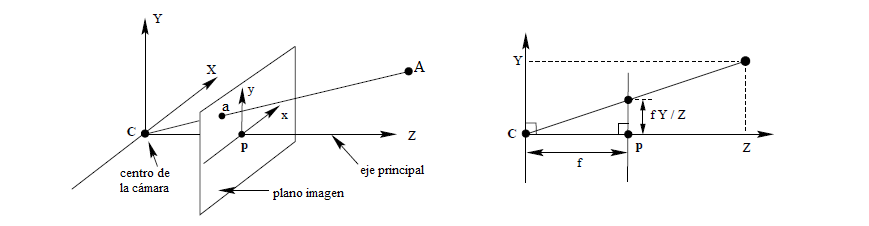
\includegraphics[width=0.8\textwidth]{./Cap2_videomapping/pinhole.png}
  \caption{Geometría de cámara \emph{pinhole}. $C$ es centro de la cámara y $p$ el punto principal}
  \label{fig:Calib-Pinhole}
\end{figure}

Un punto en el espacio $A=(A_X, A_Y, A_Z)^T$ se corresponde con el punto $a$ en el plano imagen, dado por la intersección del rayo que pasa por el centro de cámara y el punto $A$ con el plano imagen. El punto $A$ se corresponde con $(\frac{fA_X}{A_Z}, \frac{fA_Y}{A_Z}, f)^T$ en el plano imagen considerando que el centro de coordenadas del plano imagen coincide con el punto principal $P$.

Considerando la representación de los puntos como vectores homogéneos se expresa la proyección central como una correspondencia lineal entre las coordenadas homogéneas.

\[
\begin{pmatrix}
A_X \\ A_Y \\ A_Z \\ 1
\end{pmatrix}
\to
\begin{pmatrix}
fA_X \\ fA_Y \\ A_Z
\end{pmatrix}
=
\begin{pmatrix}
f & 0 & 0 & 0 \\
0 & f & 0 & 0 \\
0 & 0 & 1 & 0 \\
\end{pmatrix}
\begin{pmatrix}
A_X \\ A_Y \\ A_Z \\ 1
\end{pmatrix}
\]

Dado $A_h = (A_X,A_Y,A_Z,1)^T$ y la proyección $a$ sobre el plano imagen, la correspondencia utilizando el método pinhole es:
$a=PA_h$

Siendo
\[
P = 
\begin{pmatrix}
f & 0 & 0 & 0 \\
0 & f & 0 & 0 \\
0 & 0 & 1 & 0 \\
\end{pmatrix}
\]

\section{Geometría epipolar}
\cite{LibroCompGrafica3} La geometía epipolar es la geometía proyectiva intrínseca entre dos puntos de vista. Es dada por la intersección de los planos imagen de cada cámara con el plano epipolar, este plano es el definido por el punto a representar $X$ y los dos centros de las cámaras $C$ y $C'$.

\begin{figure}[H]
  \centering
    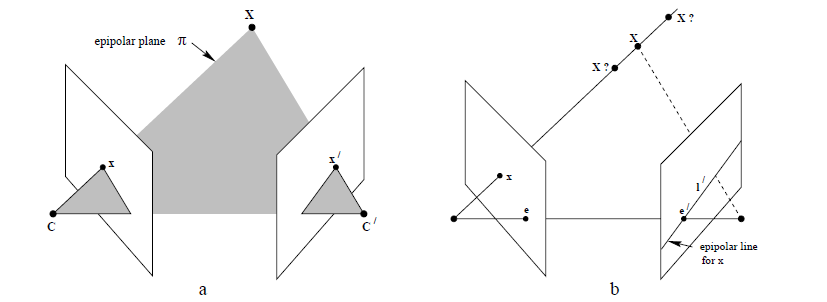
\includegraphics[width=0.7\textwidth]{./Cap2_videomapping/epipolar.PNG}
  \caption{geometía epipolar, $C$ y $C'$ centos de las cámaras.}%Geometía de Cámaras  StereoReview pag 241. fig 9.1%
  \label{fig:Epipolar}
\end{figure}
La matriz fundamental $F$ es la representación algebraica de la geometía epipolar.
Dado un par de imágenes, como se muestra en la figura para cada punto $x$ en una imagen existe una linea epipolar correspondiente $l'$ en la otra imagen. Cualquier punto $x'$ en la segunda imagen que corresponde al punto $x$ debe pertenecer a la linea epipolar $l'$.
La línea epipolar $l'$ en la segunda imagen es la proyección en la segunda imagen del rayo que parte del punto $x$ y llega al centro $C$ de la primer cámara. Hay un mapeo de un punto en una imagen con la línea epipolar en la otra imagen.
\[  x \to l'
\]
 
El mapeo en proyectiva de puntos a líneas es representado por $F$ la matriz fundamental.

\begin{figure}[H]
  \centering
    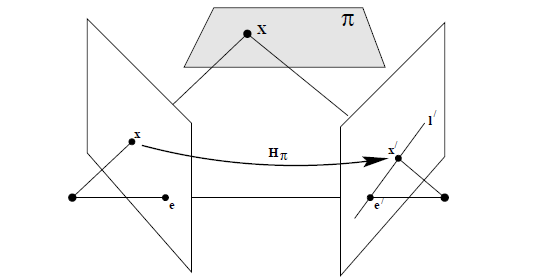
\includegraphics[width=0.7\textwidth]{./Cap2_videomapping/epipolar2.PNG}
  \caption{geometía epipolar, matriz fundamental $F$.} %Geometía de Cámaras  StereoReview pag 243. fig 9.5%
  \label{fig:Epipolar2}
\end{figure}
Dado $x$ en una imagen se corresponde con el punto $x'$ en la segunda imagen vía una trasferencia establecida por la intersección del plano $\pi$ con los planos imagen de cada cámara.
La línea epipolar que contiene $x'$ se obtiene uniendo $x'$ con el epipolo $e'$, esto es:
\[ x' = H_{\pi} * x \]    siendo  $H_{\pi}$ una homografía 2D que establece la correspondencia entre cada $x_i$ de la primer imagen a $x'_i$ en la segunda imagen.
\[ l' = e' * x' = e' * H_{\pi} * x = F * x  \]
\[ F = e' * H_{\pi}  \mbox{es la matriz fundamental}  \]